\documentclass[11pt, a4paper]{article}
\usepackage[utf8x]{inputenc}
\usepackage[sort]{natbib}

\usepackage[spanish]{babel}
\usepackage{enumitem}
\usepackage{graphicx}
\usepackage{float}
\usepackage[linktoc=all]{hyperref}

\usepackage{etoolbox}

\usepackage{amsmath}
\usepackage{amssymb}
\usepackage{array}
\usepackage{gensymb}

\usepackage{fancyhdr}
\usepackage[table]{xcolor}
\usepackage{color}
\usepackage{colortbl}
\definecolor{lightgray}{gray}{0.9}
\setlength{\columnsep}{0.5cm}


%------------------- Dimensiones -------------------
\usepackage{geometry}
 \geometry{a4paper,total={170mm,257mm},left=15mm,right=15mm,top=20mm,}
%----------------------------------------------------

%------------------- Encabezado y Pie de pág -------------------
\pagestyle{fancy}
\fancyhf{}
\lhead{Técnicas Digitales IV}
\rhead{TP1}
\rfoot{Página \thepage}
%----------------------------------------------------


%----------------------------- Documento -----------------------------------------------
\begin{document}
\begin{titlepage}
 \centering
	
\includegraphics[scale=0.80]{Imagenes/LOGO.jpg} \par
 	\vspace{1cm}
 	{\scshape\LARGE Universidad Tecnológica Nacional \par}
 	{\scshape\large Facultad Regional de Córdoba \par}
 	\vspace{1cm}
	{\bfseries \Large Trabajo Práctico De Laboratorio $N^{\circ} 1$\par}
 	\vspace{1.5cm}

	\begin{tabular}{ll}
		Della Santina, Lucas	&	66876 \\
		Navarro, Facundo		&	63809 	
	\end{tabular}
	
	\vspace{1cm}
	Curso: 6r4 \\
	Grupo $N^{\circ} 5$
 	\vfill
	{\bfseries \Large Técnicas Digitales IV\par}

	\vspace{1.5cm}
	Docentes: \par
	Ing. Cayuela, Pablo \par
	Ing. Olmedo, Sergio \par

 	\vfill
	{\large \today\par}
\end{titlepage}
	
	
\tableofcontents
\clearpage

\section{Introducción}
	El siguiente informe documenta los procedimientos realizados para el diseño digital de un controlador de un motor mediante la lectura de un encoder, se utilizar parte de las practicas adquiridas en los prácticos de entrenamiento y se profundiza en los conocimientos sobre encoders o codificadores rotativos. 

\section{Marco Teórico}
	\subsection{Encoder}
	Un ``encoder rotatorio", también llamado codificador del eje o generador de pulsos, es un dispositivo electromecánico capaz de convertir la posición angular de un eje a un código digital. Estos dispositivos se añaden suelen ser añadidos a motores de corriente continua para convertir el movimiento mecánico en pulsos digitales que pueden ser interpretado por un sistema electrónico de control. 

	Encuentran aplicación dentro de los campos de la robótica, lentes fotográficas, aplicaciones industriales que requieran medición angular, etc.

	Los motores DC tienen un comportamiento complejo en cuanto a control de posición y de la velocidad, el cual no es lineal y depende mucho de la carga que soporten, es por este motivo que surge la necesidad de la aplicación de un encoder que permita conocer y asegurar la correcta posición del eje.

	Según su diseño y funcionalidad existen distintos tipos de encoders. Los tipos mas comunes se pueden clasificar en absolutos y relativos.

	\subsubsection{Encoder Absoluto}
	Un encoder absoluto es un dispositivo que mide la posición absoluta angular. Esta diseñado para proporcionar un código digital de acuerdo a la posición angular de la flecha, como se ve en la imagen \textcolor{blue}{\textbf{\ref{fig:encoder_absoluto}}}, una vuelta esta dividida en un numero especifico de divisiones o marcas y cada una de ellas se les asigna físicamente un código digital único. Es decir que tiene un código único para cada posición. 

\begin{figure}[h]
	\centering
	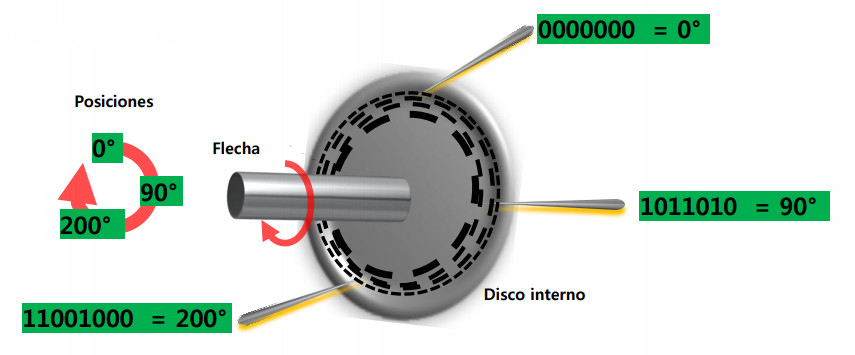
\includegraphics[width=0.8\textwidth]{Imagenes/encoder_absoluto.jpg}
	\caption{Estructura interna de un encoder absoluto.}
	\label{fig:encoder_absoluto}
\end{figure} 

\subsubsection{Encoder Incremental}
 El tipo común de encoder incremental consiste de un disco solidario al eje del motor que contiene un patrón de marcas o ranuras que son codificados por un interruptor óptico generando pulsos eléctricos cada vez que el patrón del disco interrumpe y luego permite el paso de luz hacia el interruptor óptico a medido que el disco gira. 

 Este tipo de encoders determina la posición de rotación de acuerdo  aun numero especifico de pulsos por vuelta (PPV), mediante el conteo de esos pulsos a medida que el encoder gira, es entonces que la PPV es un factor de resolución y es el aspecto mas importante a la hora de seleccionar un encoder incremental.  La resolución de un encoder típico es del orden de 1000 pulsos por revolución.

 Desde un encoder incremental no se puede determinar la posición angular absoluta del eje. Para poder determinar la posición relativa a un punto de referencia (cero), el encoder debe incluir una señal adicional que genera un pulso por revolución, denominada ``indice" (Z).

\begin{figure}[h]
	\centering
	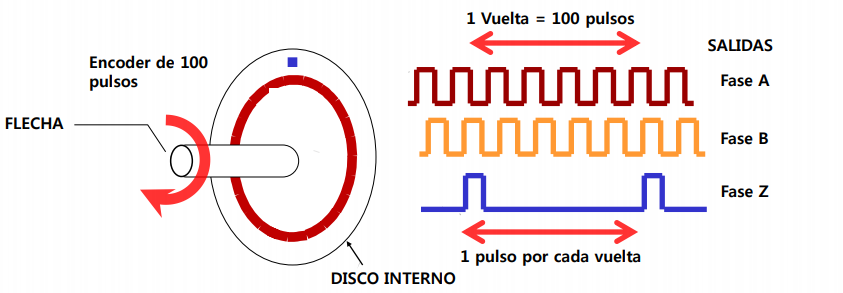
\includegraphics[width=0.8\textwidth]{Imagenes/encoder_incremental.jpg}
	\caption{Estructura interna de un encoder incremental.}
	\label{fig:encoder_incremental}
\end{figure} 

\subsubsection{Encoder en cuadratura}
Corresponde a un tipo de encoder incremental que utiliza dos sensores ópticos posicionados con un desplazamiento de 1/4 de ranura el uno del otro, generando dos señales de pulsos digitales desfasadas en 90 grados o en ``cuadratura". Estas señales se llaman comúnmente $A$ y $B$. Mediante ellas es posible suministrar los datos de posición, velocidad y dirección de rotación del eje.

Usualmente, si la señal A adelanta a B (la señal A toma un valor lógico de ``1" antes que B) se establece el convenio que el eje esta rotando en sentido horario, mientras que si B adelanta a A, el sentido anti horario, como se ve en la figura \textcolor{blue}{\textbf{\ref{fig:encoder_cuadratura}}}.
\begin{figure}[h]
	\centering
	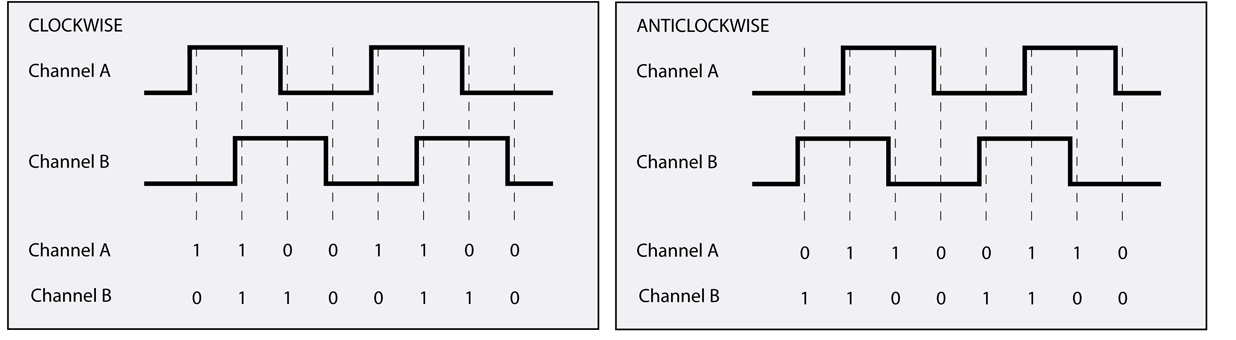
\includegraphics[width=0.8\textwidth]{Imagenes/encoder_cuadratura.jpg}
	\caption{Sentido de giro del encoder en cuadratura}
	\label{fig:encoder_cuadratura}
\end{figure} 

\section{Desarrollo}

	\subsection{Decodificador de encoder visualizando en cuatro display de 7 segmentos}
	Realizar la descripción de divisores de frecuencia para el barrido de los displays a una frecuencia de 1kHz, utilizando una clock de 15 kHz. Describir un contador decimal de 000 a 999. Incorporar el concepto de descripción jerárquico utilizando instanciación de componentes.
	Con una descripción de máquina de estado realizar la decodificación de los flancos de las señales A y B del encoder y transofromarlas en pulsos Up/Down según el sentido de giro.

		\subsubsection{Divisor de frecuencia y multiplexado de displays}
			A partir de la frecuencia de entrada $f_1$ en 15 kHz, se pretende utilizar para realizar el multiplexado de los 3 displays necesarios para visualizar la cuenta hasta 999, como el ojo no es capaz de percibir el encendido y apagado a alta velocidad, fenómeno conocido como persistencia de la visión, engañando a la espectador en creer que el los displays se encuentran encendido en simultaneo. 

		\subsubsection{Contador 0 - 999}
		
		\subsubsection{Decodificador de cuadratura}
	
		\begin{figure}[h]
			\centering
			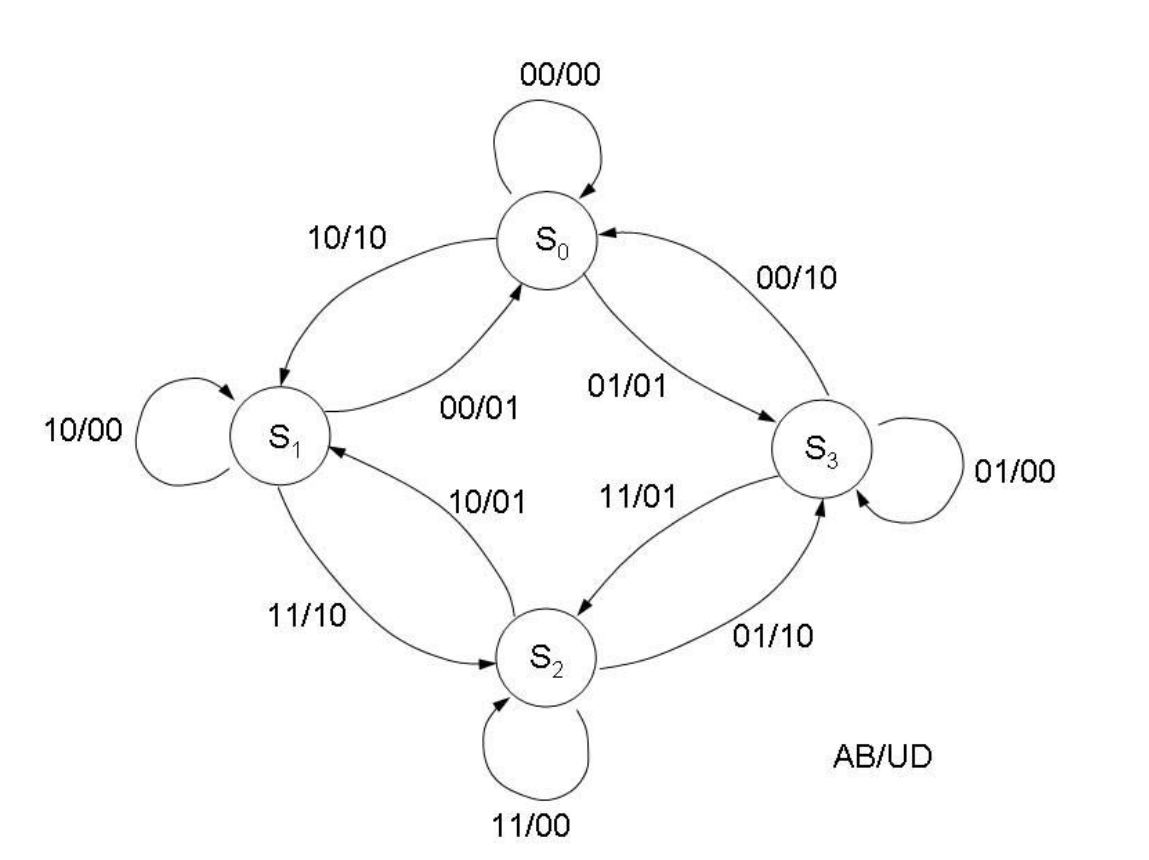
\includegraphics[width=0.8\textwidth]{Imagenes/mealy.jpg}
			\caption{Maquina de Mealy}
			\label{fig:mealy}
		\end{figure} 
	
	
	\subsection{Control de lazo de velocidad de un motor C.C.}


	\subsection{Control de motor paso a paso de velocidad a lazo abierto con rampa de aceleración y desale ración parametrizable}
\end{document}
